\RequirePackage{iftex}
\ifpdftex\else
  \errmessage{This template uses vntex (T5 font encoding) and must be compiled with pdfLaTeX, not XeLaTeX or LuaLaTeX. On Overleaf: Menu > Compiler > pdfLaTeX}
  \expandafter\stop
\fi

\documentclass[a4paper, 12pt]{article}
\newcommand{\coursename}{Data Warehouses and Decision Support Systems}
\newcommand{\coursecode}{CO4031}

\newcommand{\reportkind}{Project Report}
\newcommand{\reporttitle}{Tourism -- Hotel Revenue Management Decision Support System}

% Submission phase, shown after \reportkind on the title page. Leave it empty {} to hide it.
\newcommand{\reportphase}{}

% People listed on the title page: one person per line, separated by \\
\newcommand{\reportadvisors}{Assoc.\ Prof.\ Dr.\ Võ Thị Ngọc Châu}
\newcommand{\reportstudents}{%
  Phạm Khánh Duy (\textit{2310510}) \\
  Nguyễn Trần Yến Nhi (\textit{2312506}) \\
  Tăng Hồng Ái (\textit{2310167})}

% Author in the PDF properties
\newcommand{\reportauthor}{Phạm Khánh Duy, Nguyễn Trần Yến Nhi, Tăng Hồng Ái}

\newcommand{\reportplace}{Ho Chi Minh City}
\newcommand{\reportyear}{2026}

% "Writing guide" boxes in each subsection (see styles/guide.tex). Change to \showguidesfalse to hide all of them,
% e.g. to preview the report without them. Delete each box once its subsection is written.
\newif\ifshowguides
\showguidestrue

% Preamble: packages, page layout, header/footer and heading format.
\usepackage{
    amssymb,
    epsfig,
    latexsym,
    multicol,
    array,
    hhline,
    fancyhdr
}
\usepackage{vntex}
\usepackage[english]{babel}
\usepackage{csquotes}
\DeclareQuoteGlyph{T5}{13}
\DeclareQuoteGlyph{T5}{14}
\DeclareQuoteGlyph{T5}{15}
\DeclareQuoteGlyph{T5}{16}
\DeclareQuoteGlyph{T5}{17}
\DeclareQuoteGlyph{T5}{18}
\DeclareQuoteGlyph{T5}{19}
\DeclareQuoteGlyph{T5}{20}
\DeclareQuoteGlyph{T5}{34}
\DeclareQuoteGlyph{T5}{39}
\DeclareQuoteGlyph{T5}{96}
\usepackage{etoolbox}
\usepackage{booktabs}
\usepackage{amsmath}
\usepackage{algorithm}
\usepackage{algorithmic}
\usepackage{lastpage}
\usepackage{enumerate}
\usepackage{color}
\usepackage{graphicx}
\graphicspath{{figures/}}
\usepackage{ragged2e}
\usepackage{tabularx}
\usepackage[labelfont=bf, labelsep=colon]{caption}
\captionsetup[figure]{name=Figure}
\captionsetup[table]{name=Table}
\usepackage{multirow}
\usepackage[framemethod=tikz]{mdframed}
\usepackage{rotating}
\usepackage{graphics}
\usepackage{geometry}
\usepackage{setspace}
\usepackage{tikz}
\usetikzlibrary{arrows.meta, positioning}
\usepackage{listings}
\geometry{a4paper, top=3cm, bottom=2.5cm, left=2cm, right=2cm, headheight=10mm, headsep=5mm, footskip=10mm}

\definecolor{dkgreen}{rgb}{0,0.6,0}
\definecolor{gray}{rgb}{0.5,0.5,0.5}
\definecolor{mauve}{rgb}{0.58,0,0.82}

\usepackage{float}
\usepackage{longtable}
\usepackage{paralist}

\lstset{frame=tb, language=Python, aboveskip=3mm, belowskip=3mm,
showstringspaces=false, columns=fixed, basicstyle={\ttfamily\small}, numbers=none,
numberstyle=\tiny\color{gray},
keywordstyle=\color{blue},
commentstyle=\color{dkgreen},
stringstyle=\color{mauve},
breaklines=true, breakatwhitespace=true, tabsize=3, numbers=left, stepnumber=1,
numbersep=5pt, firstnumber=1, numberfirstline=true}

% biblatex with IEEE style
\usepackage[backend=biber, style=ieee, sorting=none]{biblatex}
\addbibresource{refs.bib}

% Header/footer: logo + university name in the header, course and page number in the footer.
% Built without tabular so that \arraystretch (changed in main.tex) cannot move the header.
% The logo sits 2.5mm below the text baseline, and the declared 4mm depth keeps a 1.5mm gap above the header rule.
\pagestyle{fancy}
\fancyhead{}
\fancyhead[L]{\raisebox{-2.5mm}[5.5mm][4mm]{
\includegraphics[width=8mm, height=8mm]{hcmut.png}}\hspace{2mm}%
\small\textbf{Ho Chi Minh City University of Technology}}
\fancyfoot{} % clear all footer fields
\fancyfoot[L]{\scriptsize \textbf{\coursename{} (\coursecode)}}
\fancyfoot[R]{\scriptsize Page {\thepage}/\pageref{LastPage}}
\renewcommand{\headrulewidth}{0.3pt}
\renewcommand{\footrulewidth}{0.3pt}




\onehalfspacing

% Guide boxes and TikZ diagram styles
% "Writing guide" boxes: what a subsection should contain and which questions it should answer.
% Delete a box once its subsection is written. \showguidesfalse in metadata.tex hides all of them at once.
\definecolor{guideaccent}{RGB}{180,83,9}
\definecolor{guidebackground}{RGB}{255,247,230}

% The box is one line of a paragraph (accent bar + \colorbox), so it never splits across pages and LaTeX keeps it on
% the same page as the heading above it. mdframed is not used here: it always adds a page break point before the box,
% which leaves the heading alone at the bottom of the page when the box moves to the next one.
\NewDocumentEnvironment{guide}{+b}{%
  \ifshowguides
    \par\addvspace{\medskipamount}%
    \begingroup
      \setlength{\fboxsep}{6pt}%
      \noindent{\color{guideaccent}\vrule width 2pt}% without a height, the rule spans the whole box
      \colorbox{guidebackground}{%
        \begin{minipage}{\dimexpr\linewidth-2pt-2\fboxsep\relax}
          \small
          {\color{guideaccent}\textbf{Writing guide}}\par
          #1
        \end{minipage}}%
      \par
    \endgroup
    \addvspace{\medskipamount}%
  \fi
}{}

% Bold label inside a guide box, e.g. \guidepart{Questions to answer}
\newcommand{\guidepart}[1]{\par\smallskip\textbf{#1}\par}

% TikZ styles for diagrams (star schema, DSS architecture, influence diagrams)
\tikzset{
    factbox/.style={rectangle, draw=blue!70!black, fill=blue!10, thick, minimum width=3.2cm, minimum height=1.2cm, align=center},
    dimbox/.style={rectangle, draw=orange!80!black, fill=orange!10, thick, minimum width=2.6cm, minimum height=0.9cm, align=center},
    sysbox/.style={rectangle, draw=teal!70!black, fill=teal!10, thick, minimum width=3.5cm, minimum height=1.3cm, align=center, rounded corners=3pt},
    arrow/.style={-{Stealth[length=3mm]}, thick},
    dasharrow/.style={-{Stealth[length=3mm]}, thick, dashed},
    label/.style={font=\small\itshape, text=gray},
}



\begin{document}

%%%%%%%%%%%%%%%%%%%%%%%%%%%%%%%%%
\pagenumbering{alph}
\begin{titlepage}
    
\begin{tikzpicture}[remember picture, overlay, inner sep=0, outer sep=0]
        \draw[blue!70!black, line width=4pt]
            ([xshift=-1.5cm,yshift=-2cm]current page.north east) coordinate (A)
            -- ([xshift=1.5cm,yshift=-2cm]current page.north west) coordinate (B)
            -- ([xshift=1.5cm,yshift=2cm]current page.south west) coordinate (C)
            -- ([xshift=-1.5cm,yshift=2cm]current page.south east) coordinate (D) -- cycle;
        \draw ([yshift=0.5cm,xshift=-0.5cm]A) -- ([yshift=0.5cm,xshift=0.5cm]B)
            -- ([yshift=-0.5cm,xshift=0.5cm]B) -- ([yshift=-0.5cm,xshift=-0.5cm]B)
            -- ([yshift=0.5cm,xshift=-0.5cm]C) -- ([yshift=0.5cm,xshift=0.5cm]C)
            -- ([yshift=-0.5cm,xshift=0.5cm]C) -- ([yshift=-0.5cm,xshift=-0.5cm]D)
            -- ([yshift=0.5cm,xshift=-0.5cm]D) -- ([yshift=0.5cm,xshift=0.5cm]D)
            -- ([yshift=-0.5cm,xshift=0.5cm]A) -- ([yshift=-0.5cm,xshift=-0.5cm]A)
            -- ([yshift=0.5cm,xshift=-0.5cm]A);
        \draw ([yshift=-0.3cm,xshift=0.3cm]A) -- ([yshift=-0.3cm,xshift=-0.3cm]B)
            -- ([yshift=0.3cm,xshift=-0.3cm]B) -- ([yshift=0.3cm,xshift=0.3cm]B)
            -- ([yshift=-0.3cm,xshift=0.3cm]C) -- ([yshift=-0.3cm,xshift=-0.3cm]C)
            -- ([yshift=0.3cm,xshift=-0.3cm]C) -- ([yshift=0.3cm,xshift=0.3cm]D)
            -- ([yshift=-0.3cm,xshift=0.3cm]D) -- ([yshift=-0.3cm,xshift=-0.3cm]D)
            -- ([yshift=-0.3cm,xshift=-0.3cm]A) -- ([yshift=0.3cm,xshift=0.3cm]A)
            -- ([yshift=-0.3cm,xshift=0.3cm]A);
    \end{tikzpicture}
    \vspace{0.25cm}
    \begin{center}
        \textbf{ĐẠI HỌC QUỐC GIA THÀNH PHỐ HỒ CHÍ MINH}\\
        \vspace{0.05cm}
        \textbf{TRƯỜNG ĐẠI HỌC BÁCH KHOA}\\
        \vspace{0.05cm}
        \textbf{KHOA KHOA HỌC VÀ KỸ THUẬT MÁY TÍNH} \\
    \end{center}
    \vspace{0.55cm}
    \begin{figure}[h!]
        \begin{center}
            
\includegraphics[scale=0.5]{hcmut.png}
        \end{center}
    \end{figure}
    \vspace{0.55cm}
    \begin{center}
        \parbox{0.9\linewidth}{\centering
            {\Large \textbf{\coursename{} (\coursecode)}}\\[0.3cm]
            \rule{0.85\linewidth}{0.5pt}\\[0.4cm]
            {\Large \textbf{\reportkind\ifdefempty{\reportphase}{}{ -- \reportphase}}}\\[0.3cm]
            {\Large \textbf{\textit{``\reporttitle''}}}
            \\[0.4cm]
            \rule{0.85\linewidth}{0.5pt}
        }
        \vspace{1cm}
        \newcommand{\stackedlines}[1]{\begin{tabular}[t]{@{}l@{}}#1\end{tabular}}
        \begin{tabular}{r l}
            \textbf{GVHD:} & \stackedlines{\reportadvisors} \\
                                 &                                \\
            \textbf{Sinh viên:} & \stackedlines{\reportstudents} \\
        \end{tabular}
    \end{center}
    \vspace{4.25cm}
    \begin{center}
        \textbf{\reportplace{} $-$ \reportyear}
    \end{center}
\end{titlepage}
\pagenumbering{arabic}
\pagebreak
\tableofcontents
\pagebreak

\addcontentsline{toc}{section}{\listfigurename}
\listoffigures
\addcontentsline{toc}{section}{\listtablename}
\listoftables
\pagebreak

\renewcommand{\arraystretch}{1.5}
\setlength{\LTpre}{0pt}
\setlength{\LTpost}{0pt}

% TODO: Acknowledgements
\section*{Acknowledgements}

We would like to express our gratitude to...


%%%%%%%%%%%%%%%%%%%%%%%%%%%%%%%%%
\section{Introduction}
\subsection{Tourism Domain and Lodging Economics}

\paragraph{Tourism and its components.}
Tourism is one of the largest industries in the world, yet it is also, in the words of Goeldner and Ritchie, ``\emph{a complex phenomenon, one that is extremely difficult to describe succinctly}'' (p.~14)~\cite{goeldner2009}. The textbook organises the phenomenon into four interrelated components --- the tourist, the natural resources and environment, the built environment, and the operating sectors of the tourism industry --- as shown in Figure~\ref{fig:tourism-phenomenon} (Fig.~1.2, p.~14).

The heart of the model is the tourist: ``\emph{the very heart of the tourism phenomenon model is unequivocally the tourist and the travel experiences that he or she seeks}'' (p.~15). For revenue management this has a direct meaning: each tourist is a decision maker who chooses whether to book a room, at what price, at what time, and through which channel. Around the tourist, the natural resources and environment of a destination --- physiography, climate, culture --- are largely immutable: they cannot be adjusted to raise visitor arrivals (p.~14)~\cite{goeldner2009}, and this immutability is the root of \emph{seasonality}. The built environment distinguishes \emph{infrastructure} --- roads, sewage systems, communication networks built to meet the needs of local residents --- from the \emph{tourism superstructure}: ``\emph{facilities that have been developed especially to respond to the demands of visitors}'' (p.~17), with hotels listed as the first example. Crucially, ``\emph{the characteristics of components of the superstructure are essentially determined by visitor wishes rather than resident desires}'' (p.~17): a hotel's pricing, room types, and services must reflect what visitors want and are willing to pay for. Finally, the operating sectors --- transportation, accommodation, food services, attractions, events, and others --- are ``\emph{what many of the general public perceive as `tourism'}'' (p.~19)~\cite{goeldner2009}; Figure~\ref{fig:operating-sectors} shows the textbook's view of these sectors. Among them, ``\emph{tourists need a place to stay and be fed, so the accommodation sector and the food service sector are important supply components}'' (p.~383)~\cite{goeldner2009}, and our problem belongs to the accommodation sector, which Chapter~6 of the textbook develops.

\begin{figure}[H]
\centering
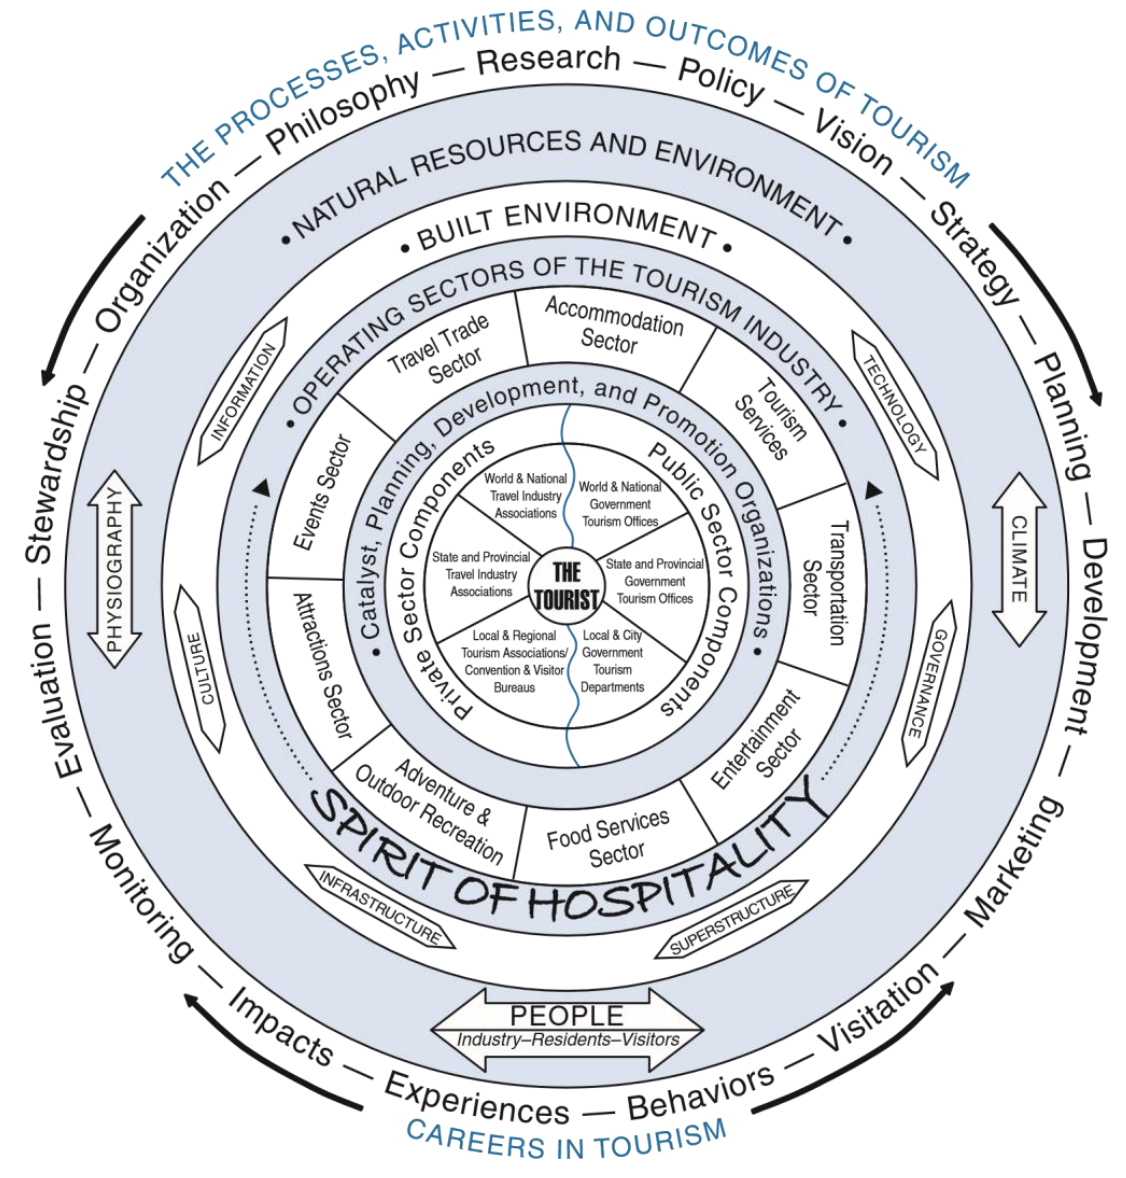
\includegraphics[width=0.52\textwidth]{figures/1-introduction/tourism-phenomenon.png}
\caption{The tourism phenomenon: components of tourism and tourism management (Goeldner \& Ritchie, Fig.~1.2, p.~14)~\cite{goeldner2009}.}
\label{fig:tourism-phenomenon}
\end{figure}

\begin{figure}[H]
\centering
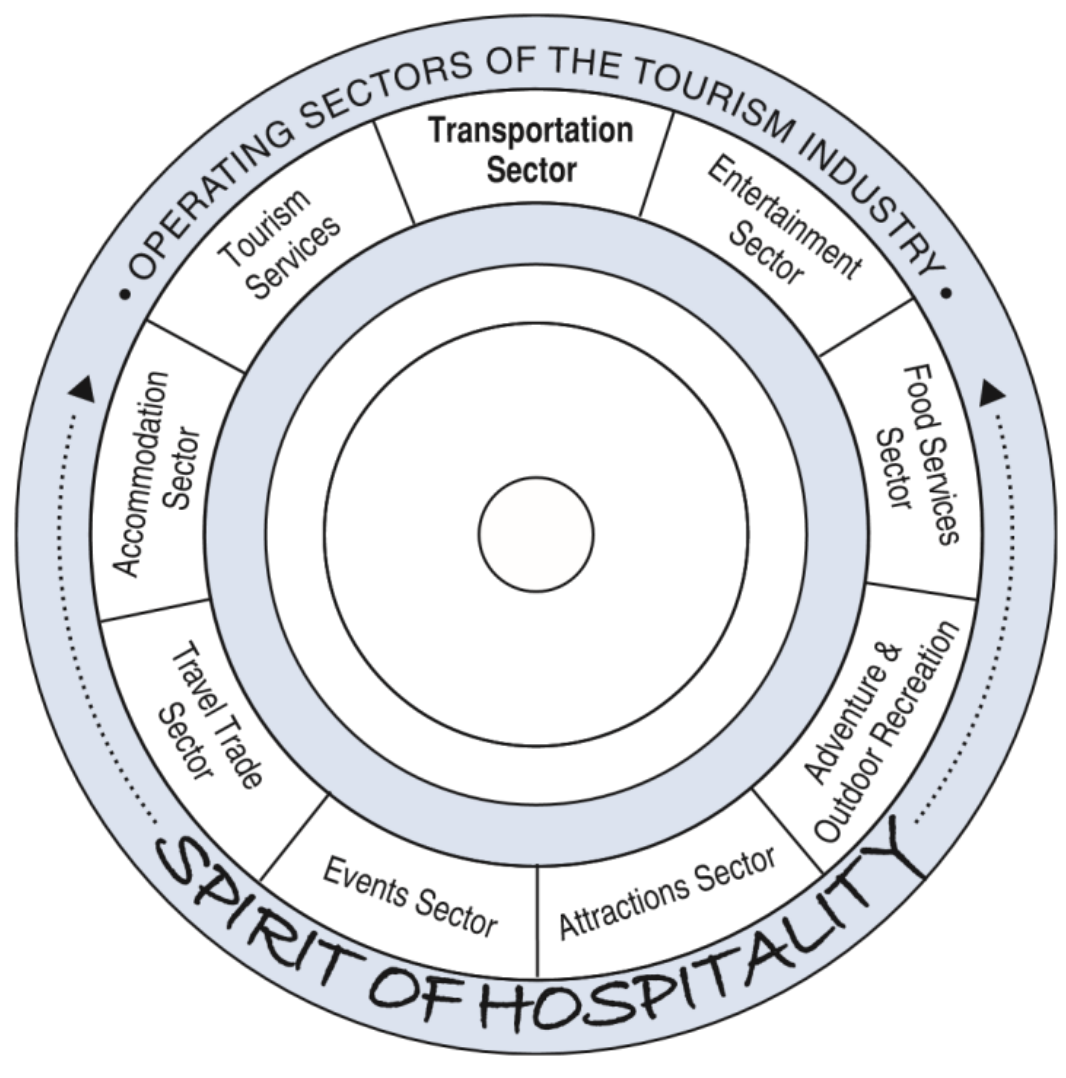
\includegraphics[width=0.5\textwidth]{figures/1-introduction/operating-sectors.png}
\caption{Operating sectors of the tourism industry --- accommodation is one of them (Goeldner \& Ritchie, Ch.~1)~\cite{goeldner2009}.}
\label{fig:operating-sectors}
\end{figure}

\paragraph{The lodging industry.}
Providing overnight accommodation ``\emph{goes back into antiquity; it is the world's oldest commercial business}'' (p.~180). The sector spans a wide range of accommodation structures --- hotels, motels, suites, resort properties, bed-and-breakfasts, timeshare, and camping (Figure~\ref{fig:accommodation-structures}; Ch.~6)~\cite{goeldner2009} --- of which our project addresses the hotel segment. The scale of the U.S.\ sector alone, per the AH\&LA 2007 Lodging Industry Profile cited in the textbook, is ``\emph{47{,}135 properties, 4.4 million rooms, \$133.4 billion in sales, \$26.6 billion in pretax profit, 63.3 percent average occupancy rate, and \$61.93 revenue per available room}'' (p.~156). An average occupancy of 63.3\% means that more than one-third of all hotel rooms go unsold every night --- a substantial, recurring revenue gap.

\begin{figure}[H]
\centering
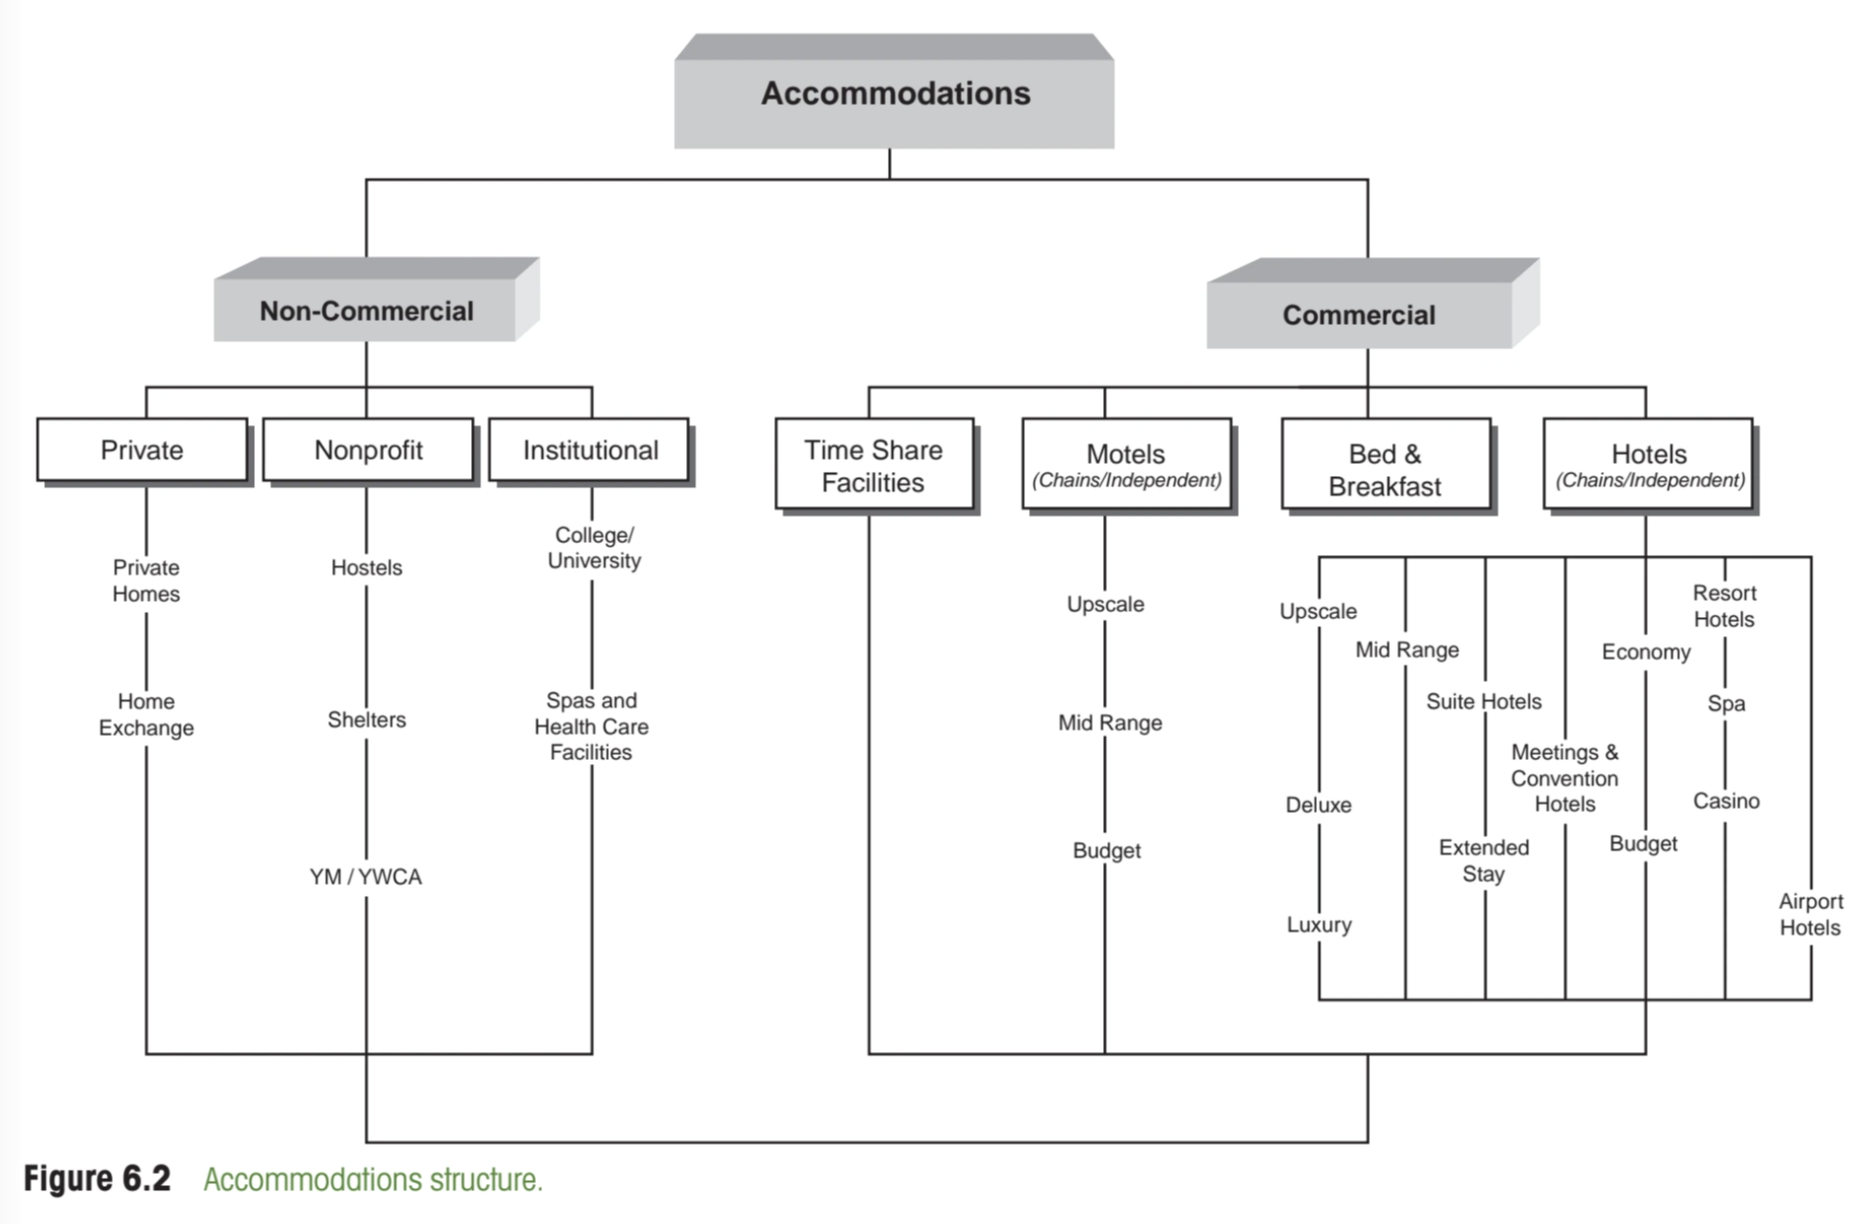
\includegraphics[width=0.7\textwidth]{figures/1-introduction/accommodation-structures.png}
\caption{Structures of the accommodation sector (Goeldner \& Ritchie, Ch.~6)~\cite{goeldner2009}.}
\label{fig:accommodation-structures}
\end{figure}

\paragraph{Key performance indicators.}
The textbook's glossary defines the three metrics that every revenue manager monitors (p.~186): \textbf{ADR} (Average Daily Rate) is ``\emph{guestroom revenue for a given period divided by total number of occupied rooms}''; \textbf{Occupancy} is ``\emph{available rooms occupied for a given period. Computed by dividing the number of rooms occupied by the number of rooms available}''; and \textbf{RevPAR} (Revenue Per Available Room) is ``\emph{guestroom revenue for a given period divided by total number of available rooms. A simple way to calculate is to multiply the occupancy times the room rate}''. These three metrics are tightly coupled: raising rates (higher ADR) may reduce occupancy, while lowering rates to fill rooms may reduce ADR. RevPAR is the composite measure that captures this trade-off, and it is the optimisation target of the system developed in this project.

\paragraph{Customer segments.}
``\emph{Who is the typical lodging customer? According to the AH\&LA, 44 percent are business travelers and 56 percent are leisure travelers}'' (p.~156). The typical business room-night is generated by a male (65\%) aged 35--54, earning \$85{,}900 per year, travelling alone (56\%), and paying \$112 per night; the typical leisure room-night involves two adults, earning \$77{,}100, travelling by automobile (77\%), and paying \$103 per night. The difference in price sensitivity and booking behaviour between these segments is the economic foundation for differentiated pricing: the same room is worth different amounts to different customers.

\paragraph{Structural characteristics of supply, cost, and demand.}
Revenue management is both necessary and difficult because six structural conditions hold simultaneously in hotel lodging, and each grounds one part of the solution developed in this project.

\emph{Product and capacity constraints.} First, the product is \textbf{perishable}: an unsold room-night cannot be stored or resold --- ``\emph{the utilization of perishable assets}''~\cite{mcgill1999}, ``\emph{the perishable nature of hotel rooms}''~\cite{amadeus2023} --- the property that drove the airline industry to originate yield management~\cite{rothstein1971} and that is shared by all capacity-constrained service businesses~\cite{kimes1989} (Table~\ref{tab:perishable}). Second, \textbf{capacity is relatively fixed}: a hotel cannot add or remove rooms on a daily basis; accommodations ``\emph{must be available in sufficient quantity to match the demand of the travelers who arrive at the destination}'' (p.~388)~\cite{goeldner2009}.

\emph{Economics and cost structure.} Third, the industry combines \textbf{high fixed costs with low variable costs}: ``\emph{the high fixed cost and low variable cost typically associated with the hotel industry means that a large portion of this revenue increase flows directly to the bottom line}''~\cite{anderson2012}. This is the economic motor of the problem: because the marginal cost of selling one more room is close to zero, every euro of revenue that pricing and allocation recover converts almost entirely into profit.

\emph{Market and booking dynamics.} Fourth, \textbf{demand fluctuates} predictably across seasons and days of the week while supply stays constant, creating excess demand in peaks and excess capacity off-peak --- an imbalance rooted, in the textbook's terms, in the immutability of a destination's natural resources (p.~14)~\cite{goeldner2009}. Fifth, demand is \textbf{segmentable}: ``\emph{RM is about a hotel's ability to segment its consumers and price and control room inventory differently across these segments --- in essence practicing some form of price discrimination}''~\cite{anderson2012}; the willingness-to-pay gap between the business and leisure segments documented above makes this concrete, and rate fences (time of purchase, refundability, affiliation) keep the segments separated~\cite{anderson2012}. Sixth, bookings occur \textbf{in advance of consumption}, across a booking window measured in days before arrival: ``\emph{RM systems use existing reservations on hand (ROH) to develop forecasts for future arrivals days}'', with booking and pace curves presented as functions of days before arrival~\cite{anderson2012}. The window is recorded in the data itself (booking lead time)~\cite{antonio2019} and is where the overbooking model of this project measures its show-up probabilities.

Together, the first four conditions explain why the problem exists --- a perishable, fixed-capacity product with near-zero marginal cost, facing uneven demand --- and the last two why it is tractable: segmentation provides the price lever, and the booking window provides the observation and intervention timeline.

\begin{table}[H]
\centering
\caption{Perishable inventory across capacity-constrained service industries~\cite{kimes1989}.}
\label{tab:perishable}
\begin{tabular}{@{}ll@{}}
\toprule
\textbf{Industry} & \textbf{Perishable inventory} \\
\midrule
Hotels & Room for a given night \\
Airlines & Seat on a given flight \\
Tours & Seat on a given departure \\
Restaurants & Table for a given service period \\
Events & Ticket for a given performance \\
\bottomrule
\end{tabular}
\end{table}

\paragraph{Measuring demand.}
Chapter~13 of the textbook frames demand measurement for tourism: ``\emph{demand for travel to a particular destination will be a function of the person's propensity to travel and the reciprocal of the resistance of the link between origin and destination areas. Thus, $D = f(\text{propensity}, \text{resistance})$}'' (p.~414). Among the possible measures, the textbook is explicit about the unit that matters for our sector: ``\emph{data on visitor-days and visitor-nights are much more valuable to tourism planners than are data on the number of arrivals}'' and ``\emph{hotel and other accommodations people want data on visitor-nights}'' (p.~418). This is the domain justification for the booking-night grain of the data warehouse designed in Section~3.2. Money spent is ``\emph{the most meaningful measure}'' but also ``\emph{the most difficult measure to obtain}'' (Ch.~13)~\cite{goeldner2009}.

\paragraph{The industry's response: yield management.}
Against this background, the textbook records the industry's response as a clear trend: ``\emph{Other trends are the increased use of central reservation systems, emphasis on service, and the use of yield management techniques}'' (p.~190). The glossary defines yield management as ``\emph{the use of pricing and inventory controls, based upon historical data, to maximize profits by offering varying fares over time for the same product}'' (p.~698), and the classic operations-management formulation states its objective plainly: ``\emph{the objective of yield management is to maximize the revenue or yield of the firm. A good yield management system will help the firm decide how much of each type of inventory (whether it be seats on an airplane, rooms in a hotel, or cars in a rental car fleet) to allocate to different types of demand}''~\cite{kimes1989}. The economics justify the effort: hotel revenue management ``\emph{has been shown to increase revenue by 2 to 5 percent}''~\cite{anderson2012}; commercial revenue management decision support systems report gains of approximately 6\%~\cite{boyd2003}, and American Airlines' pioneering system 4--7\%~\cite{smith1992}. In the language of operations research, revenue management is ``\emph{the utilization of perishable assets to maximize a firm's revenues over a short-term horizon given that costs are effectively fixed over that horizon}''~\cite{mcgill1999} --- confirming conditions 1 and 3 above (perishable inventory, and the high-fixed-cost/low-variable-cost structure) from the operations-research tradition. Contemporary industry guidance confirms that revenue management now rests on four foundational principles --- \emph{segmentation}, \emph{forecasting}, \emph{optimisation}, and \emph{distribution}~\cite{amadeus2023} --- which map directly onto the models developed in this project.

\subsection{Hotel Revenue Management}

\paragraph{Definition and goal.}
Contemporary industry guidance defines hotel revenue management as ``\emph{the process of maximizing revenue and profits through the strategic management of pricing, hotel inventory, and distribution channels}'' (tr.~5)~\cite{amadeus2023}: revenue managers analyse market demand, adjust pricing and inventory levels, and employ various techniques to optimise revenue and profit margins. Its goal is ``\emph{to achieve the right balance between occupancy and rate, ensuring that hotels are operating at maximum capacity while also charging optimal prices}'' (tr.~5)~\cite{amadeus2023} --- the same ADR--occupancy tension that RevPAR captures. The practice originated in the airline industry in the 1980s and was adopted by hospitality because of ``\emph{the perishable nature of hotel rooms and the highly competitive market}'' (tr.~7)~\cite{amadeus2023}.

\paragraph{Foundational aspects.}
Four principles structure the discipline (tr.~6)~\cite{amadeus2023}: \emph{segmentation} --- understanding and targeting customer segments based on their needs, preferences, and willingness to pay; \emph{forecasting} --- predicting future demand for rooms and adjusting prices and inventory accordingly; \emph{optimisation} --- finding the optimal pricing and inventory mix to maximise revenue and profits; and \emph{distribution} --- managing sales channels so that rooms are sold through the most effective channels. Three of the four map one-to-one onto the components of this project: forecasting and optimisation become the model base of Section~3, and segmentation becomes the dimensional backbone of the warehouse; distribution is the axis our dataset cannot support, and it is treated as a documented limitation.

\paragraph{Market segments.}
The industry segments travellers into leisure, business, and group business (tr.~8--10)~\cite{amadeus2023}. Leisure demand is analysed by looking back at which traveller types the hotel has been successful with and forward at booking behaviours; business demand is cultivated proactively through local businesses, trade organisations, and convention bureaus; ``bleisure'' travellers blend business and leisure stays; and group business --- the focus of our allocation problem --- has its own tactics, from dedicated group pricing to partnerships with event planners, and a distinctly longer booking window than individual reservations.

\paragraph{Pricing strategies.}
Pricing optimisation is ``\emph{finding the optimal price for each room type, taking into account market demand, competitor pricing, and guest preferences}'' (tr.~11)~\cite{amadeus2023}. In practice it combines \emph{dynamic pricing} --- adjusting rates in real time based on demand, ``\emph{capitaliz[ing] on high-demand periods and attract[ing] price-sensitive customers during low-demand periods}'' --- with length-of-stay and value-added pricing (tr.~11)~\cite{amadeus2023}. Two monitoring concepts recur throughout the guidance: the \emph{booking window} (``\emph{continuously monitor the booking window across your most profitable segments}'', tr.~12) and \emph{pace} (``\emph{leverage occupancy pace data instead of annualized occupancy metrics}'', tr.~12)~\cite{amadeus2023}, both computed as functions of days before arrival. These are exactly the quantities our forecasting and overbooking models consume.

\paragraph{High-quality data.}
Because forecasting drives every downstream decision, the industry is explicit about what qualifies as good data. Five attributes define the standard (tr.~18)~\cite{amadeus2023}: \emph{on-the-books} (``\emph{data that is a confirmed hotel reservation, not a forecast}''), \emph{forward-looking} (business already booked for future stay dates, not a projection), \emph{sanctioned} (``\emph{extracted in partnership with the provider}''), \emph{segmented} (with ``\emph{significant depth levels of segmentation, market, and traveler attributes}''), and \emph{fresh} (``\emph{refreshed frequently, preferably daily}''). The dataset used in this project satisfies the sanctioned and segmented attributes; the on-the-books, forward-looking, and fresh attributes are addressed by design compromises discussed in Section~5.

\paragraph{Technology: the revenue management system.}
Technology matters for four reasons --- data management, forecasting and pricing, distribution, and automation --- and its most significant embodiment is the revenue management system (RMS): software that ``\emph{helps hoteliers analyze demand patterns, optimize pricing strategies, and maximize revenue by automating the process of analyzing data and adjusting room rates}'', using algorithms that account for ``\emph{seasonality, market demand, competitor pricing, and historical data}'' (tr.~22)~\cite{amadeus2023}. Viewed from industry practice, the system built in this project is a miniature RMS: a warehouse replacing the data engine, a model base replacing the algorithms, an interactive interface replacing the recommendation layer --- with the model management subsystem --- the course-adopted topic, introduced in Section~1.3 --- as the ``S'' that turns analytical models into managed, reproducible software. To avoid losing the revenue gap identified in Section~1.1, revenue management must therefore rest on data and models --- that is, on a decision support system.

\subsection{The Role of Data Warehousing and DSS in Revenue Management}

\paragraph{From transactions to analysis.}
The intellectual premise of this project is stated by the textbook itself: ``\emph{increasingly, the success of a destination is determined by its ability to assemble, interpret, and utilize information in an effective manner}'' (p.~18)~\cite{goeldner2009}. A hotel's property management system (PMS) records booking transactions as they occur, but it is an operational system: it is organised to register each booking, not to answer analytical questions such as how occupancy and ADR evolved by market segment over two years. A data warehouse fills this role --- it \emph{remembers}: it integrates historical transactions and reorganises them into dimensional facts that can be rolled up, drilled down, sliced, and diced along the analytical dimensions~\cite{kimball2013}.
The integration problem is not hypothetical: recent reviews report that privacy-driven policies against sharing guest data have produced ``\emph{siloed storage for each property, leading to the unavailability of a 360-degree view of the customer}''~\cite{jawabreh2026} --- precisely the condition a warehouse exists to remedy.

\paragraph{Revenue management runs on decision support systems.}
In commercial practice, revenue management is executed by decision support systems, not by hand. State-of-the-art systems perform explicit price optimisation, overbooking, and allocation in sequence, fed by demand forecasting~\cite{pimentel2019}, and their adoption is associated with revenue gains of approximately 6\%~\cite{boyd2003} (American Airlines' pioneering system reported 4--7\%~\cite{smith1992}). The three decisions are quantitative at their core: forecasting demand by segment, setting protection levels between fare classes (the two-class closed form dates to Littlewood~\cite{littlewood2005}), valuing capacity through bid prices, and balancing oversell against undersell costs. Running these algorithms on real data --- rather than on intuition or spreadsheets, whose ``success is largely dependent on the caliber of the person''~\cite{anderson2012} --- is precisely what a decision support system provides. Turban et al.~characterise a DSS as combining a data management subsystem, a model management subsystem, a user interface, and a knowledge-based component~\cite{turban2011}; our architecture (Section~3.1) follows this decomposition.

\paragraph{The data foundation.}
The project is grounded in real data: the hotel booking demand dataset of Antonio et al.~\cite{antonio2019}, extracted directly from the PMS databases of two Portuguese hotels (a resort in the Algarve and a city hotel in Lisbon) and described fully in Section~2. Beyond its industry specificity, the dataset was constructed with an anti-leakage principle that matches the needs of decision models: variable values were recorded as of the day prior to each arrival, so each record is an on-the-books snapshot rather than a post-hoc summary --- the same temporal discipline our overbooking model adopts (Section~3.3).
The dataset has itself already supported a published decision support system for cancellation prediction~\cite{antonio2019dss}, and a survey of public alternatives found no hotel dataset richer in revenue-management variables: every public ``hotel booking'' dataset traces back to it, and its direct successor --- four hotels, 2014--2023, 670{,}343 bookings --- is available only under NDA~\cite{silvestre2025}.

\paragraph{The course-adopted topic: the MBMS.}
The course-adopted topic for this group is the \emph{Model Base Management Subsystem} (MBMS) --- the component that manages, manipulates, and runs the models embedded in the DSS. Turban et al.~describe it as ``a module that theoretically has capabilities similar to those of a DBMS to manage, manipulate, and run the models embedded in the DSS''~\cite{turban2011}, and no standard, off-the-shelf MBMS exists: every DSS team designs its own~\cite{turban2011}. Our design --- presented in depth in Section~3.4 --- implements the model base as database tables: a \texttt{model\_catalog} of model metadata, a uniform execution registry, and a scenario run log.

\subsection{Scope and Report Organization}

\paragraph{Objectives.}
The objective of this project is to build a \emph{decision support system} (DSS) for hotel revenue management, utilising a data warehouse and data analytics as required by the course specification. The system supports a revenue manager in making three recurring tactical decisions --- pricing, group-versus-transient allocation, and overbooking --- defined precisely in Section~2. For each decision, the system produces measurable outputs aligned with the three key performance indicators of the lodging industry~\cite{goeldner2009} --- ADR, occupancy, and RevPAR. The application is interactive: the user can adjust model parameters (price levels, group allocation, overbooking thresholds) and immediately observe the resulting changes in projected KPIs through \emph{what-if analysis}, \emph{sensitivity analysis}, and \emph{goal seeking} --- the three analysis modes that Turban et al.~identify as core DSS capabilities~\cite{turban2011}.

\paragraph{Scope.}
In scope: a dimensional data warehouse built from the Antonio et al.~dataset~\cite{antonio2019}; a model base of five declared models managed by a model base management system (MBMS) --- the core of the model management subsystem (the course-adopted topic); and an interactive web application exposing the models to the decision maker. Out of scope, for reasons established in this section: distribution-channel management and competitor pricing (the dataset carries no channel commissions or competitor rates --- pricing optimisation's ``competitor pricing'' input~\cite{amadeus2023} cannot be supported); function-space, restaurant, and ancillary revenue (room revenue only~\cite{goeldner2009}); and real-time operation (the dataset is a static historical research extract rather than daily-refreshed data~\cite{amadeus2023}).

\paragraph{Report organization.}
The remainder of the report is organised as follows. Section~2 defines the business problem: the organisational context, the decision makers, the three recurring decisions and their classification, the data, and the expected goals. Section~3 presents the proposed solution: the DSS architecture, the star schema of the data warehouse, the model catalog, and the model management subsystem presented in depth. Section~4 describes the application development, Section~5 evaluates the solution, and Section~6 concludes the report.


\section{Business Problem Definition}
\subsection{Problem Statement}
\begin{guide}
  \guidepart{Nội dung cần có}
  \begin{itemize}
    \item Decision makers: revenue manager (cô Lan) + giám đốc vận hành
    \item 3 quyết định: (1) giá theo hạng/ngày, (2) phân bổ đoàn/lẻ, (3) overbooking
    \item Vì sao semistructured: máy tính làm được phần số, người phán đoán phần còn lại
    \item Dataset: 119,390 bookings, 32 columns, 2015--2017
  \end{itemize}
\end{guide}
\subsection{Expected Goals}
\begin{guide}
  \guidepart{Nội dung cần có}
  \begin{itemize}
    \item Mục tiêu chính: tối đa RevPAR
    \item Mục tiêu phụ: giảm phòng trống mùa thấp
    \item Ràng buộc: số walk $\leq$ ngưỡng
  \end{itemize}
\end{guide}

\section{Proposed Solution}
\subsection{DSS Architecture}

\paragraph{Overview.}
The proposed system follows the classical four-component DSS architecture of Turban et al.~\cite{turban2011}: a \emph{data management subsystem} (the data warehouse and its ETL pipeline), a \emph{model management subsystem} (the model base and its management software---our assigned topic, detailed in Section~3.4), a \emph{user interface subsystem} (an interactive web application), and a \emph{knowledge-based subsystem} (domain knowledge recorded as structured metadata). Figure~\ref{fig:architecture} shows how the components fit together.

\begin{figure}[H]
\centering
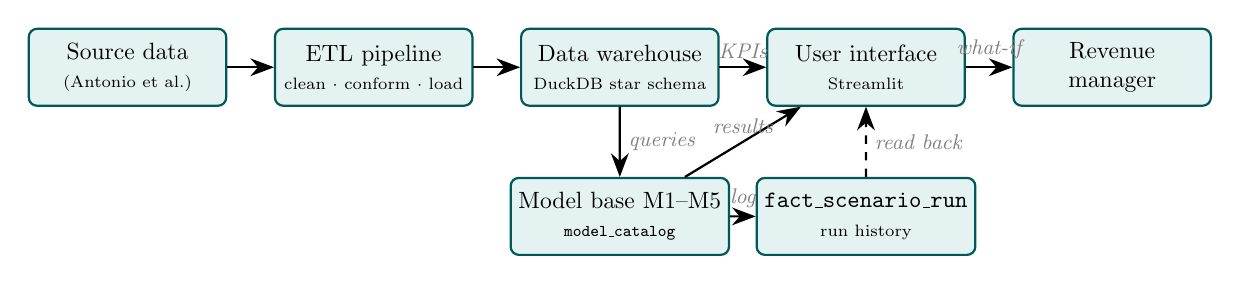
\begin{tikzpicture}[scale=0.85, every node/.style={transform shape},
  sysbox/.append style={minimum width=2.95cm, minimum height=1.15cm}]
  \node[sysbox] (src)  {Source data\\ \scriptsize (Antonio et al.)};
  \node[sysbox] (etl)  [right=0.7cm of src] {ETL pipeline\\ \scriptsize clean $\cdot$ conform $\cdot$ load};
  \node[sysbox] (dw)   [right=0.7cm of etl] {Data warehouse\\ \scriptsize DuckDB star schema};
  \node[sysbox] (ui)   [right=0.7cm of dw] {User interface\\ \scriptsize Streamlit};
  \node[sysbox] (user) [right=0.7cm of ui] {Revenue\\ manager};
  \node[sysbox] (mb)   [below=1.05cm of dw] {Model base M1--M5\\ \scriptsize \texttt{model\_catalog}};
  \node[sysbox] (run)  [below=1.05cm of ui] {\texttt{fact\_scenario\_run}\\ \scriptsize run history};

  \draw[arrow] (src) -- (etl);
  \draw[arrow] (etl) -- (dw);
  \draw[arrow] (dw) -- node[label, above]{KPIs} (ui);
  \draw[arrow] (ui) -- node[label, above]{what-if} (user);
  \draw[arrow] (dw) -- node[label, right]{queries} (mb);
  \draw[arrow] (mb) -- node[label, above]{results} (ui);
  \draw[arrow] (mb) -- node[label, above]{log} (run);
  \draw[dasharrow] (run) -- node[label, right]{read back} (ui);
\end{tikzpicture}
\caption{Overall architecture of the proposed DSS. Solid arrows show the data and control flow; the dashed arrow shows the scenario-comparison screen reading back past runs.}
\label{fig:architecture}
\end{figure}

\paragraph{Data management subsystem.}
The foundation is a Kimball-style data warehouse built with DuckDB from the booking dataset of Antonio et al.~\cite{antonio2019}. A separate warehouse is necessary because the operational source behaves like an online transaction processing (OLTP) system: it records individual booking transactions as they occur and is not organised to answer analytical questions such as ``\emph{how did the resort's August occupancy and ADR evolve by market segment over two years?}''. The data warehouse, by contrast, \emph{remembers}: it integrates and reorganises historical transactions into the dimensional star schema of Section~3.2, whose facts can be rolled up, drilled down, sliced, and diced along the analytical dimensions. The extract--transform--load (ETL) pipeline cleans the source records, conforms them into the dimensions, and asserts referential integrity and reconciliation totals before the warehouse is accepted~\cite{kimball2013,hoffer2016}.

\paragraph{Model management subsystem.}
The model base contains the five quantitative models of Section~3.3: demand forecasting (M1), the Littlewood group decision rule (M2), linear-programming allocation (M3), overbooking (M4), and pricing goal seeking (M5). Turban et al. characterise the model management software as a module with capabilities analogous to those of a DBMS, but applied to models rather than to data~\cite{turban2011}. We take this analogy literally and implement the model base itself as \emph{database tables}: a \texttt{model\_catalog} that stores each model's metadata (purpose, variable roles, assumptions, limitations) and a \texttt{fact\_scenario\_run} table that records every execution. This design is the subject of Section~3.4.

\paragraph{User interface subsystem.}
The revenue manager interacts with the system through a Streamlit web application with four screens: a KPI dashboard (ADR, occupancy, and RevPAR by hotel, period, and segment), a forecasting screen, an optimisation and what-if screen that exposes the parameters of all five models as interactive controls, and a scenario-comparison screen that reads previous runs back from the warehouse. The interface supports the three analysis modes that Turban et al. identify as core DSS capabilities~\cite{turban2011}: \emph{what-if analysis} (change a parameter, observe the projected KPIs), \emph{sensitivity analysis} (tornado charts showing which parameter the decision is most exposed to), and \emph{goal seeking} (invert the pricing model to find the rate that achieves a target RevPAR).

\paragraph{Knowledge-based subsystem.}
Rather than a full expert system, the knowledge component is deliberately lightweight: the domain knowledge that would otherwise be scattered across code comments is recorded as structured, queryable metadata. This includes the season definition (peak, shoulder, low), the classification of market segments into group versus transient business, the documented assumptions of every model (walk cost, price elasticity), and the capacity-estimation rule described in Section~3.2. Encoding these as data rather than code means every assumption is visible to the decision maker in the interface, and every result can be traced back to the assumptions that produced it.

\paragraph{A compound DSS covering all decision phases.}
In the taxonomy of Turban et al.~\cite{turban2011}, the system is a compound DSS: its dashboard is data-driven (OLAP over the star schema), while its optimisation and what-if screens are model-driven. Mapping the architecture onto Simon's four phases of decision making confirms the coverage of the problem defined in Section~2: \emph{intelligence} is served by the dashboard queries over the warehouse; \emph{design} is served by the model base, which generates candidate pricing, allocation, and overbooking alternatives; \emph{choice} is served by the optimisation and goal-seeking runs that rank those alternatives on projected RevPAR; and \emph{implementation review} is served by the scenario run log, which preserves every parameter set and outcome so that past decisions can be audited and learned from.

\subsection{Star Schema Design}
\begin{guide}
  \guidepart{Content to include}
  \begin{itemize}
    \item Kimball 4-step design: business process $\to$ grain $\to$ dimensions $\to$ facts
    \item Grain: booking-night (1 row = 1 night $\times$ 1 booking)
    \item Goeldner p.~419: ``Hotel and other accommodations people want data on visitor-nights''
    \item fact\_room\_night + fact\_daily\_occupancy + 7 dims
    \item Star schema diagram (figure)
  \end{itemize}
\end{guide}
\subsection{Model Catalog}
\begin{guide}
  \guidepart{Nội dung cần có}
  \begin{itemize}
    \item M1 Forecasting (Holt-Winters): dự báo nhu cầu theo mùa
    \item M2 Optimization (LP/PuLP): phân bổ phòng đoàn/lẻ
    \item M3 Overbooking (cost model): mức bán vượt tối ưu
    \item Mỗi model khai báo 4 loại biến (decision, uncontrollable, intermediate, result)
    \item Mỗi model khai báo static/dynamic + certainty/risk/uncertainty + cấp quản lý
  \end{itemize}
\end{guide}
\subsection{Model Base Management Subsystem}

This subsystem is the topic assigned to our group, and this section presents it in depth against the full theory: the five elements of the model management subsystem, the functions of the MBMS, the model directory, execution and integration, model selection, and the six required capabilities --- each mapped to our concrete design.

\paragraph{The five elements.}
Turban et al.\ specify the composition of the model management subsystem: it ``\emph{is composed of the following elements}: \emph{model base, MBMS, modeling language, model directory, [and] model execution, integration, and command processor}''~\cite{turban2011}. We implement each element explicitly:

\begin{itemize}
  \item \textbf{Model base} --- the collection of quantitative models that ``\emph{provide the analysis capabilities in a DSS}''~\cite{turban2011}: our five declared models of Section~3.3, plus the \emph{model building blocks and routines} the theory describes --- the regression and smoothing routines of \texttt{statsmodels}, the solver of PuLP, and the optimisation and statistics routines of SciPy --- which are exactly the kind of reusable components (``\emph{random-number generator, curve- or line-fitting routine, present-value computational routine, and regression analysis}'') the theory lists as the contents of a model base.
  \item \textbf{MBMS} --- the management software itself: our registry, described below.
  \item \textbf{Modeling language} --- the means by which models are built; because ``\emph{DSS deals with semistructured or unstructured problems, it is often necessary to customize models, using programming tools and languages}''~\cite{turban2011}, our models are written in Python against a declared interface: each module exposes a run function whose parameter schema is declared in the catalog, so that models can be invoked, combined, and replaced without touching the callers.
  \item \textbf{Model directory} --- ``\emph{a catalog of all the models and other software in the model base. It contains model definitions, and its main function is to answer questions about the availability and capability of the models}''~\cite{turban2011}: this is precisely our \texttt{model\_catalog} table, whose rows carry each model's purpose, variable declaration, parameters, assumptions, and limitations.
  \item \textbf{Model execution, integration, and command processor} --- execution is ``\emph{the process of controlling the actual running of the model}''; integration is ``\emph{combining the operations of several models when needed (e.g., directing the output of one model, say forecasting, to be processed by another one, say a linear programming planning model)}''~\cite{turban2011}: our single entry point \texttt{run\_model(model\_id, params)} controls execution for every caller, and the M1$\to$M2/M3 chaining of Section~3.3 is exactly the integration the theory describes.
\end{itemize}

\paragraph{The four functions of the MBMS.}
The MBMS software ``\emph{has four main functions}: \emph{model creation, using programming languages, DSS tools and/or subroutines, and other building blocks; generation of new routines and reports; model updating and changing; [and] model data manipulation}''~\cite{turban2011}. Our design provides each: \emph{creation} --- a new model joins the suite by writing one Python module against the declared interface and inserting one row into \texttt{model\_catalog}, reusing the building blocks (statsmodels, PuLP); \emph{generation of new routines and reports} --- every scenario run produces a structured result row that the comparison screen turns into reports, and combinations of runs (baseline vs.\ alternative) are new analyses without new code; \emph{updating and changing} --- the catalog row versions a model's declaration and assumptions, so a change is visible, comparable, and revertible; \emph{data manipulation} --- parameters are injected at run time through the registry, which is precisely what makes what-if analysis possible without touching model code.

\paragraph{Model directory details.}
Beyond the definition, the directory answers ``\emph{questions about the availability and capability of the models}''~\cite{turban2011}. Our \texttt{model\_catalog} is queried by the interface to list what models exist, what each answers, and what parameters each accepts; its capability descriptions are what the decision maker reads before choosing a model, and what the run registry validates parameters against.

\paragraph{Model selection.}
Which model to use for which situation ``\emph{cannot be done by the MBMS because it requires expertise and therefore is done manually}''~\cite{turban2011}; our design keeps selection manual --- the revenue manager chooses --- but assists it through the catalog: each row's \emph{purpose} field states the business question the model answers, which is exactly the information a selector needs. The subtler distinction the theory draws --- model selection versus \emph{solution-method selection} (which algorithm solves a chosen model class) --- is handled once at design time: M2 and M4 use closed-form critical ratios because their structure is two-class and single-period, M3 uses an LP solver because the week-level allocation problem has no closed form, and these choices are recorded in the catalog rather than re-decided per run.

\paragraph{Why there is no standard to adopt.}
Turban et al.\ are explicit that ``\emph{model management is an extremely difficult task}'' --- there are hundreds of model classes and many solution algorithms within each class, models are used in different ways in different organisations, and therefore ``\emph{MBMS are generally unique for each type of problem being solved}''; unlike DBMS, there is no standard MBMS~\cite{turban2011}. The corollary for our project is that the model management layer must be designed, not installed --- and its design is the mapping below.

\paragraph{Design: the DBMS analogy, taken literally.}
We take the analogy at the heart of the definition --- an MBMS should relate to models as a DBMS relates to data --- and implement the model base as database tables inside the same DuckDB warehouse that holds the business facts, giving the MBMS a catalog, an execution interface, and a log:

\begin{itemize}
  \item \textbf{\texttt{model\_catalog} --- the directory.} One row per model: identifier, purpose, mathematical type, classification, the four variable roles, parameters, assumptions, limitations, module path, and references. Where a DBMS catalog stores the schema of every table, ours stores the ``\emph{schema}'' of every model.
  \item \textbf{A run registry --- the execution and command processor.} A single entry point, \texttt{run\_model(model\_id, params)}, validates the parameters against the catalog entry, imports the module recorded there, executes the model, and returns structured results. Every caller --- the Streamlit interface, the experiment scripts, the test suite --- goes through the same entry point.
  \item \textbf{\texttt{fact\_scenario\_run} --- the log.} One row per execution: model identifier, scenario name, the full parameter set (JSON), the result (JSON), and the headline KPI --- the memory of every what-if, and the substrate for the comparison reports.
\end{itemize}

A folder of Python modules has none of that: no catalog, no uniform invocation, no run record --- and practice confirms the failure mode, since hotels running revenue management on ``\emph{a series of Excel spreadsheets}'' see success ``\emph{largely dependent on the caliber of the person}'' responsible~\cite{anderson2012}.

\paragraph{The six required capabilities, met one by one.}
The course summarises the expected capabilities of an MBMS as six~\cite{turban2011}; Table~\ref{tab:mbmscaps} maps each to the concrete mechanism in our design.

\begin{table}[H]
\centering
\caption{The six MBMS capabilities and their implementation in this project.}
\label{tab:mbmscaps}
\begin{tabularx}{\textwidth}{@{}l X@{}}
\toprule
\textbf{Capability} & \textbf{How our design provides it} \\
\midrule
Control & All models run exclusively through \texttt{run\_model()}; parameters are validated against the catalog before execution; the model suite is covered by automated tests with known-answer cases (for example, the Littlewood protection level and the overbooking critical ratio on textbook instances). \\
Flexibility & Models compose: M1's forecasts parameterise M2 and M3; any parameter can be overridden at run time to create a what-if scenario; a new model joins the suite by adding a module and a catalog row, without touching the interface or the registry. \\
Feedback & Every run returns its result variables together with the assumptions recorded in its catalog entry; the interface displays the change against a named baseline scenario, so the manager sees not only the number but the direction and size of the move. \\
Interface & The same registry serves the interactive UI, the batch experiment scripts, and the tests --- models contain no interface code, and the interface contains no model logic, so neither duplicates the other. \\
Redundancy reduction & Each model exists exactly once, as one canonical module referenced by its catalog row; analytical SQL over the warehouse is likewise defined once in views that the UI and the models share. \\
Increased consistency & The same model version with the same parameters produces the same results wherever it is run; every result row in \texttt{fact\_scenario\_run} carries its parameter set, so any number in the report can be traced to the run that produced it and reproduced by re-running it. \\
\bottomrule
\end{tabularx}
\end{table}

\paragraph{Why implementing the model base as data matters.}
Three practical consequences follow from treating models as managed data rather than as code. First, \emph{assumptions become visible and centralised}: the walk-cost multiple, the price elasticity, and the capacity estimate are declared once, in the catalog and the dimensions, instead of hiding in source files. Second, \emph{decisions become reproducible}: because each run logs its parameters and results, the comparison screen can answer the retrospective question that Simon's implementation phase poses --- which alternative was chosen, and why. Third, \emph{the reporting stays honest}: a model whose backtest shows it losing to a simple baseline is reported as such, because the run log preserves the comparison rather than the narrative. These are the same reasons organisations built databases in the first place, transposed from data to models.

\section{Application Development}
\subsection{ETL Pipeline}
\begin{guide}
  \guidepart{Nội dung cần có}
  \begin{itemize}
    \item Extract: đọc CSV (pandas)
    \item Transform: ghép 4 cột arrival $\to$ date, tách booking-night, mã hóa surrogate keys
    \item Load: nạp vào DuckDB star schema
    \item Sơ đồ pipeline + screenshot DuckDB
  \end{itemize}
\end{guide}
\subsection{Model Implementation}
\begin{guide}
  \guidepart{Nội dung cần có}
  \begin{itemize}
    \item M1: statsmodels ExponentialSmoothing, train 2015--2016, test 2017
    \item M2: PuLP LP, biến + ràng buộc + objective function
    \item M3: cost model, công thức break-even $p \geq C/(ADR + C)$
    \item Registry: JSON + run(model\_id, params)
    \item Code snippets quan trọng
  \end{itemize}
\end{guide}
\subsection{Streamlit User Interface}
\begin{guide}
  \guidepart{Content to include}
  \begin{itemize}
    \item 4 screens: Dashboard (OLAP), Model Catalog (MBMS), What-if/Goal-seeking, Tracking
    \item Screenshots of each screen
    \item User flow following Simon's 4 phases
  \end{itemize}
\end{guide}
\subsection{Technology Stack}
\begin{guide}
  \guidepart{Nội dung cần có}
  \begin{itemize}
    \item Bảng: công cụ $\times$ vai trò $\times$ lý do chọn
    \item Python + DuckDB + statsmodels + PuLP + Streamlit + Plotly
    \item Trade-off: vì sao không dùng Excel/Power BI
  \end{itemize}
\end{guide}
\section{Evaluation}
\subsection{Model Performance}

The evaluation methodology is designed against the quality rubric of the field: a 2026 systematic review of machine intelligence in hospitality identifies three recurring weaknesses --- overreliance on simulations, limited external validation, and incomplete reporting of cross-validation and benchmarking~\cite{jawabreh2026} --- and our design addresses each. Every model is evaluated on \emph{out-of-sample} data (rolling backtests, not in-sample fits); every method is compared against \emph{explicit baselines} (seasonal-naive forecasts; no-overbooking and accept-all policies); and \emph{uncertainty is reported} (Monte Carlo confidence intervals, tornado sensitivities).

\paragraph{M1: forecasting backtest.}
The backtest uses rolling monthly cut-off points across the data window: at each cut-off, only data up to that date is visible to the model, and the following 28 days are forecast. The error metrics --- MAE (mean absolute error in room-nights), RMSE, and WAPE (weighted absolute percentage error) --- are computed for every method (Holt--Winters, repeat-last-week, same-week-last-year, year-over-year scaled) on the same windows. The winner is the method with the lowest error on the test hotel's data, and the report presents the full comparison table. If a seasonal-naive baseline wins, the report says so --- the honest-evaluation discipline that the field evidence supports: in a recent multi-property study, simple exponential smoothing was the most accurate method in four of eleven tested horizons~\cite{yeoman2024}.

\paragraph{M2: worked group-decision example.}
The Littlewood rule is evaluated on a concrete scenario rather than an abstract accuracy metric, because its output is a decision, not a prediction. The demonstration presents a group request (a specified number of rooms for a specified number of nights at a specified discount ratio) against the forecast demand for each property and each season. The expected-revenue difference between accepting and rejecting is computed, and the breakeven group rate --- the rate at which the two alternatives are indifferent --- is reported. The scenario is run for both hotels in both peak and off-peak seasons, showing that the same request can be accepted in one context and rejected in another --- the essence of the tactical allocation decision.

\paragraph{M3: allocation and bid prices.}
The LP is demonstrated on a week-long scenario with several competing group offers, each spanning different nights and room types. The solver's output is presented in three forms: the optimal total revenue; the accepted set of groups; and the bid prices --- the dual values of the capacity constraints per (night, room type), which are the marginal revenue value of one more room. The demonstration shows that the shadow price of a fully utilised room type equals or exceeds its transient rate (the room is the binding constraint), while unconstrained nights have a shadow price of zero (the room is not scarce).

\paragraph{M4: overbooking with replay verification.}
The overbooking model is evaluated in two ways. First, the critical-ratio computation is verified on a known-answer instance and cross-checked by Monte Carlo simulation (20{,}000 replications, fixed seed, 95\% confidence interval). Second, a \emph{replay evaluation} runs the historical booking data forward in chronological order, applying three alternative booking-limit policies --- no overbooking ($L = C$), optimal overbooking ($L = B^{*}$ at each cut-off), and accept-all --- and compares the resulting net revenue (revenue minus walk costs) over the evaluation window. The replay uses real historical bookings, not simulated demand, and is run at three capacity levels (the estimated capacity, plus stress levels at 90\% and 80\%) because the estimated capacity is never exceeded in the historical data --- a censored-observation limitation. The results are reported honestly: if the data does not support a strong overbooking claim at the true capacity level, the report says so.

\paragraph{Sensitivity of $B^{*}$.}
The overbooking model's output is presented with a sensitivity analysis showing how the optimal booking limit moves as the cancellation rate, the walk-cost multiple, and the capacity change. This is the \emph{sensitivity analysis} mode the theory defines --- ``\emph{attempts to assess the impact of a change in the input data or parameters on the proposed solution}''~\cite{turban2011}.

\subsection{What-if Demonstration}
\begin{guide}
  \guidepart{Content to include}
  \begin{itemize}
    \item S1: cancellation/no-show rate rises 5 points $\to$ new $B^{*}$ and overbooking level (both hotels)
    \item S2: group request (rooms $\times$ nights at a discount ratio) $\to$ accept/reject per hotel with $\Delta$ revenue
    \item S3: RevPAR target $+20\%$ in low season $\to$ required ADR + occupancy loss + tornado on elasticity
    \item S4: weekly allocation with several competing group requests $\to$ accepted set + shadow prices
    \item Demo scenario following Simon's 4 phases; what-if screenshot (slider $\to$ chart update); goal-seeking screenshot
    \item Scenario comparison table read from \texttt{fact\_scenario\_run}
  \end{itemize}
\end{guide}
\subsection{Limitations and Assumptions}
\begin{guide}
  \guidepart{Content to include}
  \begin{itemize}
    \item Total rooms not available $\to$ estimated from max(rooms\_sold)
    \item adr = 0 $\to$ complimentary rooms, need filtering
    \item Revenue = room revenue only (no F\&B)
    \item 2 hotels in different segments $\to$ run models separately
    \item Canceled bookings: distinguish demand vs revenue
  \end{itemize}
\end{guide}
\section{Conclusion}
\subsection{Summary}
\begin{guide}
  \guidepart{Nội dung cần có}
  \begin{itemize}
    \item Tóm tắt: đã xây dựng gì, đạt được gì
    \item Điểm mạnh: DW + MBMS + 3 models + interactive UI
  \end{itemize}
\end{guide}
\subsection{Future Work}
\begin{guide}
  \guidepart{Content to include}
  \begin{itemize}
    \item Extensions: recapture modelling of turned-away demand, elasticity estimation (A/B tests or external data), annual seasonality (needs more years of data), richer knowledge-based subsystem, SCD Type 2, more business areas (spa, F\&B), real-time data sources
  \end{itemize}
\end{guide}

%%%%%%%%%%%%%%%%%%%%%%%%%%%%%%%%%
\printbibliography[heading=bibintoc, title={References}]
\end{document}
